\documentclass[9pt,xcolor=table,svgnames]{beamer}
\usepackage{showcode}
% \usetheme{adapt-lab}
\usetheme{customadapt-lab}

% \usepackage{MnSymbol}
\let\Square\undefined
\usepackage{bbding}
\usepackage{pifont}
\usepackage{txfonts}

\usepackage{tabularx}
% \usepackage{bibentry}
\usepackage{booktabs}
\usepackage{tikz}

\usepackage{media9}

\usetikzlibrary{angles,shadows.blur,positioning,backgrounds}
\usepackage[dvipsnames]{xcolor}
\usepackage{amsmath}
\usepackage{amssymb}
\newcommand{\globalminwidth}{15cm}
\newcommand{\globalminheight}{12cm}
\newcommand{\scopeminwidth}{((\globalminwidth - 1cm) / 2 - 0.5cm)}
\newcommand{\scopeminheight}{(\globalminheight / 3)}


\title[Toward a Modular Approach for TSs and LSP generation]{Toward a Modular Approach for Type Systems and LSP generation}
% \author{Federico Cristiano Bruzzone}
% \institute{Università degli Studi di Milano \\
%            Facoltà di Scienze e Tecnologie \\
%            Corso di Laurea Magistrale in Informatica \\ [5pt]\vspace{15pt}
%            {\normalsize Advisor: Prof. Walter Cazzola} \\ [1pt]\vspace{5pt}
%            {\normalsize Co-Advisor: Dr. Luca Favalli}}
% \date{July 15\textsuperscript{th} 2024}

\author[Federico Bruzzone]
{\vspace{-10pt}Federico Bruzzone\\\vspace{7pt}{\scriptsize Id. Number: 27427A}}
\institute{\small
	Universit\`a degli Studi di Milano\\
	Computer Science Department\\
	MSc in Computer Science\\\vspace{10pt}
	\begin{tabular}{r l}
        Advisor: & Prof. Walter Cazzola \\
		Co-Advisor: & Dr. Luca Favalli \\
	\end{tabular}
}
\date{\scriptsize{15/07/2024\\\vspace{5pt}LM-18 - Computer science\\Academic Year 2023-2024}}

\tolerance=10
\emergencystretch=\maxdimen
\hyphenpenalty=10000
\hbadness=10000

\begin{document}

\begin{frame}
	\titlepage
\end{frame}

\section{Problem Statement}

\subsection[ ]{Programming Language Implementation}
\begin{frame}{\secname}
    \framesubtitle{\subsecname}
    The implementation of a programming language is a complex task that involves several implementation aspects, such as:

    \begin{tabular}{p{0.5\textwidth} p{0.5\textwidth}}
        \begin{itemize}
            \item Syntax and semantics definition
            \item \alert{Type system definition}
            \item Code generation
        \end{itemize}
        &
        \begin{itemize}
            \item Error handling and recovery
            \item \alert{IDE support}
            \item Documentation
        \end{itemize}
    \end{tabular}

    \pause

    % \huge
    It is usually done in a \alert{monolithic} way, where all the aspects are tightly coupled.

    \pause
    \bigskip

    \normalsize This makes the \alert{maintainability}, \alert{extensibility} and \alert{reusability} of the implementation difficult.
\end{frame}


\subsection[ ]{Type Systems and IDEs Support}
\begin{frame}{\secname}
    \framesubtitle{\subsecname}

    Often some parts of compilation, such as code generation, makes use of {\color{BloodRed} feature-oriented programming} to support different architectures.

    \bigskip
    \pause

    % \huge
    However, the type system and the IDE support are usually implemented using a \alert{top-down} approach.
\end{frame}


% ============================================================================

\section[SPLs]{Software Product Lines}
\subsection[ ]{}

\begin{frame}{\secname}
    \framesubtitle{\subsecname}

    Since 1990s, researchers have been working on the concept of \alert{Software Product Lines} (SPLs) to move towards a more \alert{modular} world.

    \bigskip
    \pause

    \begin{itemize}
        \item SPLs defines a \alert{family} of software products.
        \item SPLs is described by a \alert{Feature Model}.
        \item A Feature Model describes the \alert{variability} of the software.
        \item SPL \alert{variants} are generated by selecting a set of features.
        \item A \alert{feature} (or \alert{artifact}) is a first-class entity in SPLs.
    \end{itemize}
\end{frame}

\subsection[LPLs]{Language Product Lines}
\begin{frame}{\secname}
    \framesubtitle{\subsecname}
    Applying the concept of SPLs to programming languages, we obtain the concept of \alert{Language Product Lines} (LPLs).

    \bigskip
    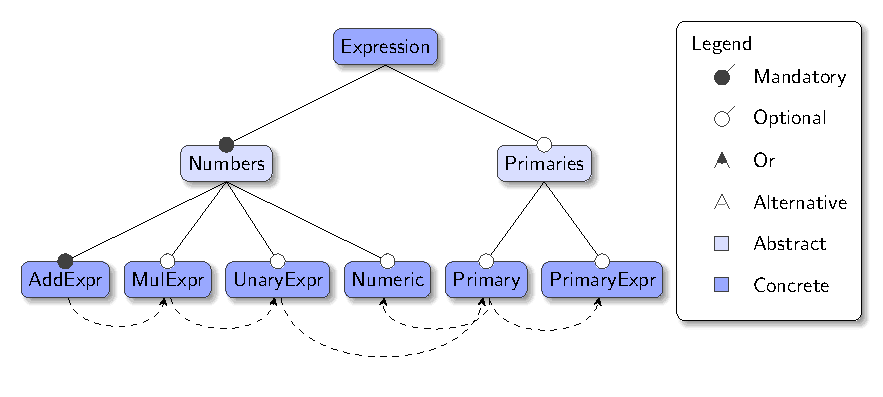
\includegraphics[width=1\textwidth]{figs/feature-model.pdf}

    \pause

    \huge Some achievements:
    \begin{itemize}
        \item \alert{Bottom-up} approach to language implementation
        \item \alert{Reusability} of language artifacts
        \item Multiple \alert{variants} of the same language
        \item \alert{Language Workbenches} come to the rescue
    \end{itemize}
\end{frame}

\subsection[LWs]{Language Workbenches and Neverlang}
\begin{frame}{\secname}
    \framesubtitle{\subsecname}

    \alert{Language Workbenches} (LWs) are tools that allow the development of programming languages, both GPLs and DSLs.

    \scriptsize Some LWs allow the development of LPLs.

    \bigskip
    \begin{table}[t]
        \rowcolors{1}{white}{gray!25}
        % \setlength\arrayrulewidth{-1pt}
        \centering
        \resizebox{\textwidth}{!}{%
        \begin{tabular}{ c c c c c c }
            \toprule \textbf{Language Workbench} & \textbf{Modularization Supp.} & \textbf{Precompiled Feature Supp.} & \textbf{Native IDE gen.} & \textbf{LSP Gen.} & \textbf{LSP Mod.} \\
            \midrule
            JustAdd & \LEFTcircle & \Circle & \Circle & \Circle & \Circle \\
            Melange & $\circledwedge$ & \Circle  & 2rd party (EMF) & \ding{80} & \ding{80} \\
            MontiCore & \LEFTcircle & \LEFTcircle & \CIRCLE & \Circle & \Circle \\
            MPS & $\circledwedge$ & \Circle   & \CIRCLE & \ding{80} & \ding{80} \\
            Rascal & \Circle & \Circle & \CIRCLE & \Circle & \Circle \\
            Spoofax & $\circledwedge$  & \LEFTcircle  & \CIRCLE & \ding{80} & \ding{80} \\
            Xtext & \Circle & \LEFTcircle  & \CIRCLE & \CIRCLE & \Circle \\
            Neverlang & $\circledvee$ & \CIRCLE & \Circle & \FiveStarConvex & \FiveStarConvex \\
            \bottomrule
        \end{tabular}
        }
        % \caption{Comparison of language workbenches in terms of modularization, precompiled feature support, native IDE generation, LSP generation, and LSP modularization. The $\CIRCLE$ symbol indicates full support, $\Circle$ no support, $\LEFTcircle$ limited support, $\circledvee$ fine-grained modularization,  $\circledwedge$ coarse-grained modularization, \FiveStarConvex my expected contribution and \ding{79} my expected contribution that can be extended to all LWs that support at least component modularization.}
        \label{tab:lw-comparison}
    \end{table}

    \bigskip
    \begin{tabular}{p{0.5\textwidth} p{0.5\textwidth}}
    \begin{itemize}
        \item[{\color{black}\CIRCLE}] Full support
        \item[{\color{black}\Circle}] No support
        \item[{\color{black}\LEFTcircle}] Limited support
        \item[{\color{black}$\circledvee$}] Fine-grained mod.
    \end{itemize}
    &
    \begin{itemize}
        \item[{\color{black}$\circledwedge$}] Coarse-grained mod.
        \item[{\color{black}\FiveStarConvex}] My contribution
        \item[{\color{black}\ding{80}}] Future Work
   \end{itemize}
   \end{tabular}

    \pause

    \normalsize \alert{Neverlang} is a language workbench, developed by the \alert{ADAPT} lab, that supports the development of LPLs.

\end{frame}

\section[LSP]{Language Server Protocol}

\subsection[The Reductions of Combinations]{The Reduction of Combinations}
\begin{frame}{\secname}
    \framesubtitle{\subsecname}

    In 2016, \alert{Microsoft} in collaboration with \alert{Red Hat} introduced the \alert{Language Server Protocol} (LSP).

    \pause
    \begin{center}
    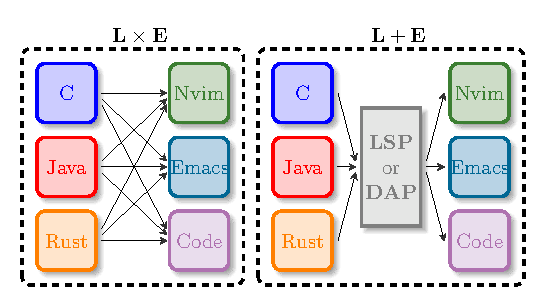
\includegraphics[width=0.8\textwidth]{figs/lsp-combination.pdf}
    \end{center}

    \pause

    \huge Spoiler:
    \normalsize We have reduced the number of combinations from $\mathbf{L} \times \mathbf{E}$ to $\mathbf{N} \times \mathbf{1}$ where $\mathbf{N} \ll \mathbf{L}$.
\end{frame}

\subsection[In a Nutshell]{LSP In a Nutshell}
\begin{frame}{\secname}
    \framesubtitle{\subsecname}

    The \alert{Language Server Protocol} (LSP) is a protocol that allows the communication between a \alert{Language Server} and an \alert{IDE}.

    \pause

    \begin{center}
    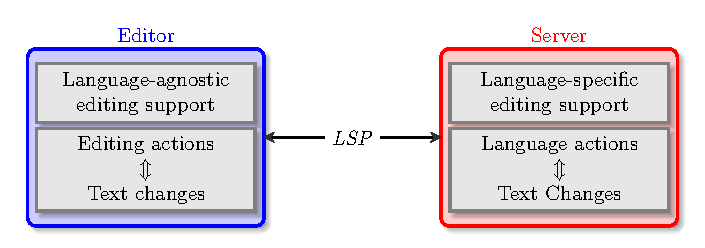
\includegraphics[width=0.8\textwidth]{figs/lsp-diagram.pdf}
    \end{center}

    \begin{tabular}{p{0.5\textwidth} p{0.5\textwidth}}
    Intrinsic properties:
    \begin{itemize}
        \item Language-agnostic
        \item IDE-agnostic
        \item Asynchronous
        \item Text-based
    \end{itemize}
        &
    Features:
    \begin{itemize}
        \item Diagnostics
        \item Hover
        \item Go to definition
        \item Find references
        \item Inlay hints
    \end{itemize}
    \end{tabular}
\end{frame}

% ============================================================================

\section[Contribution]{Contribution}

\subsection[Type System Components]{Type System Components}

\begin{frame}{\secname}
    \framesubtitle{\subsecname}
    % 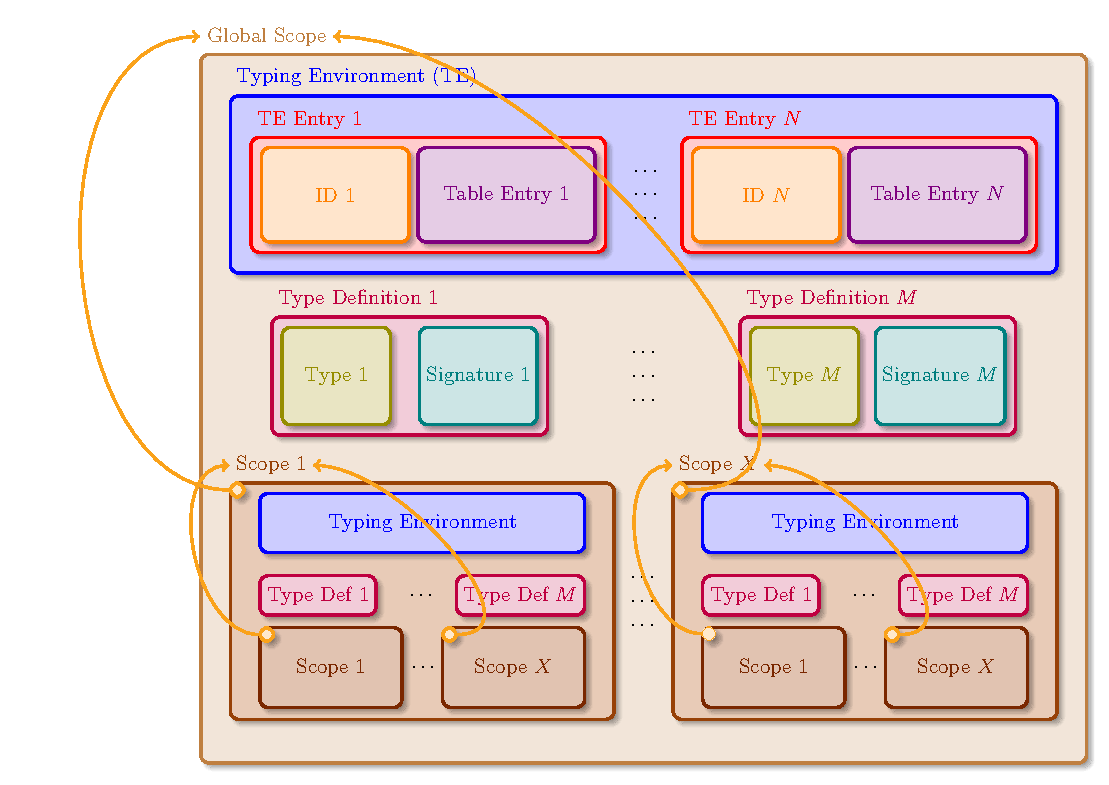
\includegraphics[width=0.8\textwidth, left]{figs/type-system.pdf}

    \resizebox{0.8\textwidth}{!}{
    \begin{tikzpicture}

    % FIRST TRY
    % \node[draw, very thick, rounded corners, fill=Black!10, blur shadow={shadow blur steps=5}, minimum width=10cm, minimum height=6cm] (LV) {};
    % \node[] (LV_label) [above right=0cm and 0cm of LV.north west] {Language Variant};

    % SECOND TRY
    % \node[draw, rectangle, very thick, rounded corners, fill=Black!10, blur shadow={shadow blur steps=5}, minimum width=10cm, minimum height=6cm, label={[above left=0pt]Language Variant}] (LV) {};

    % THIRD TRY
    \node[draw=brown,
          rectangle,
          very thick,
          rounded corners,
          fill=brown!20,
          blur shadow={shadow blur steps=5},
          minimum width=\globalminwidth,
          minimum height=\globalminheight] (GS) at (0,0) {};
    \node[text=brown, above right] (GST) at (GS.north west) {Global Scope};

    % ====================================================================
    \uncover<2->{
    \node[draw=blue,
          text=blue,
          rectangle,
          very thick,
          rounded corners,
          fill=blue!20,
          blur shadow={shadow blur steps=5},
          minimum width=\globalminwidth - 1cm,
          minimum height=\globalminheight / 4,
          below=20pt] (TE) at (GS.north) {};
    \node[text=blue, above right]  at (TE.north west) {Typing Environment (TE)};
    }

    \uncover<3->{
       \node[draw=red,
          text=red,
          rectangle,
          very thick,
          rounded corners,
          fill=red!20,
          blur shadow={shadow blur steps=5},
          minimum width=(\globalminwidth - 1cm) / 2 - 1cm,
          minimum height=(\globalminheight / 4) - 30pt,
          below right=20pt and 10pt] (TE1) at (TE.north west) {};
        \node[text=red, above right] at (TE1.north west) {TE Entry $1$};

    \node[draw=orange,
          text=orange,
          rectangle,
          very thick,
          rounded corners,
          fill=orange!20,
          blur shadow={shadow blur steps=5},
          minimum width=((\globalminwidth - 1cm) / 2 - 1cm) / 2 - 0.5cm,
          minimum height=((\globalminheight / 4) - 30pt) - 10pt,
          below right=5pt and 5pt] (TEID1) at (TE1.north west) {ID $1$};
    \node[draw=violet,
          text=violet,
          rectangle,
          very thick,
          rounded corners,
          fill=violet!20,
          blur shadow={shadow blur steps=5},
          minimum width=((\globalminwidth - 1cm) / 2 - 1cm) / 2,
          minimum height=((\globalminheight / 4) - 30pt) - 10pt,
          below left=5pt and 5pt] (TEE2) at (TE1.north east) {Table Entry $1$};


    % dots
    \node[right=0.325cm] (Dots1) at (TE1.east) {$\cdots$};
    \node[above] (Dots2) at (Dots1.north) {$\cdots$};
    \node[below] (Dots3) at (Dots1.south) {$\cdots$};

    \node[draw=red,
          text=red,
          rectangle,
          very thick,
          rounded corners,
          fill=red!20,
          blur shadow={shadow blur steps=5},
          minimum width=(\globalminwidth - 1cm) / 2 - 1cm,
          minimum height=(\globalminheight / 4) - 30pt,
          below left=20pt and 10pt] (TEN) at (TE.north east) {};
    \node[text=red, above right] at (TEN.north west) {TE Entry $N$};

    \node[draw=orange,
          text=orange,
          rectangle,
          very thick,
          rounded corners,
          fill=orange!20,
          blur shadow={shadow blur steps=5},
          minimum width=((\globalminwidth - 1cm) / 2 - 1cm) / 2 - 0.5cm,
          minimum height=((\globalminheight / 4) - 30pt) - 10pt,
          below right=5pt and 5pt] (TEIDN) at (TEN.north west) {ID $N$};

    \node[draw=violet,
          text=violet,
          rectangle,
          very thick,
          rounded corners,
          fill=violet!20,
          blur shadow={shadow blur steps=5},
          minimum width=((\globalminwidth - 1cm) / 2 - 1cm) / 2,
          minimum height=((\globalminheight / 4) - 30pt) - 10pt,
          below left=5pt and 5pt] (TEEN) at (TEN.north east) {Table Entry $N$};
      }

    % ====================================================================
    \uncover<4->{
    \node[draw=purple,
          text=purple,
          rectangle,
          very thick,
          rounded corners,
          fill=purple!20,
          blur shadow={shadow blur steps=5},
          minimum width=(\globalminwidth - 1cm) / 3,
          minimum height=\globalminheight / 6,
          below right=20pt and 20pt] (TS1) at (TE.south west) {};
    \node[text=purple, above right] at (TS1.north west) {Type Definition $1$};
    % \node<1>[text=purple, above right] at (TS1.north west) {Type Definition $1$};
    % \node<2>[text=purple, above right, fill=red] at (TS1.north west) {Type Definition $1$};

    \node[draw=olive,
          text=olive,
          rectangle,
          very thick,
          rounded corners,
          fill=olive!20,
          blur shadow={shadow blur steps=5},
          minimum width=(((\globalminwidth - 1cm) / 3) / 2) - 0.5cm,
          minimum height=(\globalminheight / 6) - 10pt,
          below right=5pt and 5pt] (TY1) at (TS1.north west) {Type $1$};

     \node[draw=teal,
          text=teal,
          rectangle,
          very thick,
          rounded corners,
          fill=teal!20,
          blur shadow={shadow blur steps=5},
          minimum width=(((\globalminwidth - 1cm) / 3) / 2) - 0.5cm,
          minimum height=(\globalminheight / 6) - 10pt,
          below left=5pt and 5pt] (SGN1) at (TS1.north east) {Signature $1$};


    % dots
    \node[right=(\globalminwidth - 1cm) / 11] (Dots1) at (TS1.east) {$\cdots$};
    \node[above] (Dots2) at (Dots1.north) {$\cdots$};
    \node[below] (Dots3) at (Dots1.south) {$\cdots$};

    \node[draw=purple,
          text=purple,
          rectangle,
          very thick,
          rounded corners,
          fill=purple!20,
          blur shadow={shadow blur steps=5},
          minimum width=(\globalminwidth - 1cm) / 3,
          minimum height=\globalminheight / 6,
          below left=20pt and 20pt] (TS2) at (TE.south east) {};
    \node[text=purple, above right] at (TS2.north west) {Type Definition $M$};

    \node[draw=olive,
          text=olive,
          rectangle,
          very thick,
          rounded corners,
          fill=olive!20,
          blur shadow={shadow blur steps=5},
          minimum width=(((\globalminwidth - 1cm) / 3) / 2) - 0.5cm,
          minimum height=(\globalminheight / 6) - 10pt,
          below right=5pt and 5pt] (TY2) at (TS2.north west) {Type $M$};

    \node[draw=teal,
          text=teal,
          rectangle,
          very thick,
          rounded corners,
          fill=teal!20,
          blur shadow={shadow blur steps=5},
          minimum width=(((\globalminwidth - 1cm) / 3) / 2) - 0.5cm,
          minimum height=(\globalminheight / 6) - 10pt,
          below left=5pt and 5pt] (SGN2) at (TS2.north east) {Signature $M$};
    }

    % ====================================================================
    \node[draw=RawSienna,
          text=RawSienna,
          rectangle,
          very thick,
          rounded corners,
          fill=RawSienna!20,
          blur shadow={shadow blur steps=5},
          minimum width=\scopeminwidth,
          minimum height=\scopeminheight,
          below right=100pt and 0pt] (S1) at (TE.south west) {};
    \node[text=RawSienna, above right] (S1T) at (S1.north west) {Scope $1$};

    \node[right=0.125cm] (Dots1) at (S1.east) {$\cdots$};
    \node[above] (Dots2) at (Dots1.north) {$\cdots$};
    \node[below] (Dots3) at (Dots1.south) {$\cdots$};

    \node[draw=RawSienna,
          text=RawSienna,
          rectangle,
          very thick,
          rounded corners,
          fill=RawSienna!20,
          blur shadow={shadow blur steps=5},
          minimum width=\scopeminwidth,
          minimum height=\scopeminheight,
          below left=100pt and 0pt] (SX) at (TE.south east) {};
    \node[text=RawSienna, above right] (SXT) at (SX.north west) {Scope $X$};

    % ====================================================================

    \uncover<5->{
    \node[draw=YellowOrange,
          text=YellowOrange,
          rectangle,
          very thick,
          rounded corners,
          fill=YellowOrange!20,
          blur shadow={shadow blur steps=5},
          minimum width=0.2cm,
          minimum height=0.2cm,
          below right = 0pt and 0pt] (P1) at (S1.north west) {};
    % Arrow from P1 to GST
    \draw[YellowOrange, ->, very thick] (P1) to[out=180, in=180] (GST.west);
    }

    \uncover<2->{
    \node[draw=blue,
          text=blue,
          rectangle,
          very thick,
          rounded corners,
          fill=blue!20,
          blur shadow={shadow blur steps=5},
          minimum width=\scopeminwidth - 1cm,
          minimum height=\scopeminheight / 4,
          below=5pt] (TE) at (S1.north) {Typing Environment};
      }

    % ====================================================================
    \uncover<4->{
    \node[draw=purple,
          text=purple,
          rectangle,
          very thick,
          rounded corners,
          fill=purple!20,
          blur shadow={shadow blur steps=5},
          minimum width=(\scopeminwidth - 1cm) / 3,
          minimum height=\scopeminheight / 6,
          below right=10pt and 0pt] (TS1) at (TE.south west) {Type Def $1$};

    % dots
    \node[right=(\scopeminwidth - 2cm) / 11] (Dots1) at (TS1.east) {$\cdots$};

    \node[draw=purple,
          text=purple,
          rectangle,
          very thick,
          rounded corners,
          fill=purple!20,
          blur shadow={shadow blur steps=5},
          minimum width=(\scopeminwidth - 1cm) / 3,
          minimum height=\scopeminheight / 6,
          below left=10pt and 0pt] (TS2) at (TE.south east) {Type Def $M$};
      }

    \node[draw=Brown,
          text=Brown,
          rectangle,
          very thick,
          rounded corners,
          fill=Brown!20,
          blur shadow={shadow blur steps=5},
          minimum width=\scopeminwidth / 2.7,
          minimum height=\scopeminheight / 4 + 10pt,
          below right=35pt and 0pt] (SI1) at (TE.south west) {Scope $1$};

    \uncover<5->{
    \node[draw=YellowOrange,
          text=YellowOrange,
          rectangle,
          very thick,
          rounded corners,
          fill=YellowOrange!20,
          blur shadow={shadow blur steps=5},
          minimum width=0.2cm,
          minimum height=0.2cm,
          below right = 0pt and 0pt] (PP1) at (SI1.north west) {};
    \draw[YellowOrange, ->, very thick] (PP1) to[out=180, in=180] (S1T.west);

    \node[right=0cm] (Dots1) at (SI1.east) {$\cdots$};
    }

    \node[draw=Brown,
          text=Brown,
          rectangle,
          very thick,
          rounded corners,
          fill=Brown!20,
          blur shadow={shadow blur steps=5},
          minimum width=\scopeminwidth / 2.7,
          minimum height=\scopeminheight / 4 + 10pt,
          below left=35pt and 0pt] (SIX) at (TE.south east) {Scope $X$};

    \uncover<5->{
    \node[draw=YellowOrange,
          text=YellowOrange,
          rectangle,
          very thick,
          rounded corners,
          fill=YellowOrange!20,
          blur shadow={shadow blur steps=5},
          minimum width=0.2cm,
          minimum height=0.2cm,
          below right = 0pt and 0pt] (PPX) at (SIX.north west) {};
    \draw[YellowOrange, ->, very thick] (PPX) to[out=0, in=0] (S1T.east);
    }


    % ====================================================================

    % ====================================================================
    \uncover<5->{
    \node[draw=YellowOrange,
          text=YellowOrange,
          rectangle,
          very thick,
          rounded corners,
          fill=YellowOrange!20,
          blur shadow={shadow blur steps=5},
          minimum width=0.2cm,
          minimum height=0.2cm,
          below right = 0pt and 0pt] (P1) at (SX.north west) {};
    % Arrow from P1 to GST
    \draw[YellowOrange, ->, very thick] (P1) to[out=0, in=0] (GST.east);
    }

    \uncover<2->{
    \node[draw=blue,
          text=blue,
          rectangle,
          very thick,
          rounded corners,
          fill=blue!20,
          blur shadow={shadow blur steps=5},
          minimum width=\scopeminwidth - 1cm,
          minimum height=\scopeminheight / 4,
          below=5pt] (TE) at (SX.north) {Typing Environment};
      }


    % ====================================================================
    \uncover<4->{
    \node[draw=purple,
          text=purple,
          rectangle,
          very thick,
          rounded corners,
          fill=purple!20,
          blur shadow={shadow blur steps=5},
          minimum width=(\scopeminwidth - 1cm) / 3,
          minimum height=\scopeminheight / 6,
          below right=10pt and 0pt] (TS1) at (TE.south west) {Type Def $1$};

    % dots
    \node[right=(\scopeminwidth - 2cm) / 11] (Dots1) at (TS1.east) {$\cdots$};

    \node[draw=purple,
          text=purple,
          rectangle,
          very thick,
          rounded corners,
          fill=purple!20,
          blur shadow={shadow blur steps=5},
          minimum width=(\scopeminwidth - 1cm) / 3,
          minimum height=\scopeminheight / 6,
          below left=10pt and 0pt] (TS2) at (TE.south east) {Type Def $M$};
      }

    \node[draw=Brown,
          text=Brown,
          rectangle,
          very thick,
          rounded corners,
          fill=Brown!20,
          blur shadow={shadow blur steps=5},
          minimum width=\scopeminwidth / 2.7,
          minimum height=\scopeminheight / 4 + 10pt,
          below right=35pt and 0pt] (SI1) at (TE.south west) {Scope $1$};


    \uncover<5->{
    \node[draw=YellowOrange,
          text=YellowOrange,
          rectangle,
          rounded corners,
          fill=YellowOrange!20,
          blur shadow={shadow blur steps=5},
          minimum width=0.2cm,
          minimum height=0.2cm,
          below right = 0pt and 0pt] (PP1) at (SI1.north west) {};
    \draw[YellowOrange, ->, very thick] (PP1) to[out=180, in=180] (SXT.west);

    \node[right=0cm] (Dots1) at (SI1.east) {$\cdots$};
    }

    \node[draw=Brown,
          text=Brown,
          rectangle,
          very thick,
          rounded corners,
          fill=Brown!20,
          blur shadow={shadow blur steps=5},
          minimum width=\scopeminwidth / 2.7,
          minimum height=\scopeminheight / 4 + 10pt,
          below left=35pt and 0pt] (SIX) at (TE.south east) {Scope $X$};
    \uncover<5->{
    \node[draw=YellowOrange,
          text=YellowOrange,
          rectangle,
          very thick,
          rounded corners,
          fill=YellowOrange!20,
          blur shadow={shadow blur steps=5},
          minimum width=0.2cm,
          minimum height=0.2cm,
          below right = 0pt and 0pt] (PPX) at (SIX.north west) {};
    \draw[YellowOrange, ->, very thick] (PPX) to[out=0, in=0] (SXT.east);
    }
    \end{tikzpicture}
    }

\end{frame}

% - Type System implementation and a Java Library for Neverlang in order to support the type system for every langauge developed with Neverlang.
% - Type System Modularization
% - DSL for Type System definition
% - LSP generation for Neverlang languages
% - Client and Syntax Highlighting generation

% ============================================================================

\setbeamercolor{background canvas}{bg=black}
\section[LSP in Action]{LSP in Action}
% Movie
\begin{frame}
    {\hspace*{6cm}\vbox to 0cm {\vspace*{4cm}
\includegraphics[width=9cm]{./figs/black_rect.png}}}
    \begin{center}
    \includemedia[
      width=1\textwidth,
      height=1\textheight,
      % activate=pageopen,
      keepaspectratio,
      playbutton=plain,
      addresource=videos/LSP_in_action.webm,
      flashvars={
         source=videos/LSP_in_action.webm
         &autoPlay=false
         &loop=true
      }
    ]{}{VPlayer.swf}
    \end{center}
\end{frame}
\setbeamercolor{background canvas}{bg=white}

\section[LSP in Action]{LSP in Action}
% Movie
\begin{frame}
    HELLO
\end{frame}
% ============================================================================


% \section[Test]{Test}
% \begin{frame}
%     % \sliderust{typeinference.rs}
%     \slideneverlang*{AddExpr.nl}
% \end{frame}

\end{document}

